% Options for packages loaded elsewhere
\PassOptionsToPackage{unicode}{hyperref}
\PassOptionsToPackage{hyphens}{url}
%
\documentclass[
]{book}
\usepackage{amsmath,amssymb}
\usepackage{iftex}
\ifPDFTeX
  \usepackage[T1]{fontenc}
  \usepackage[utf8]{inputenc}
  \usepackage{textcomp} % provide euro and other symbols
\else % if luatex or xetex
  \usepackage{unicode-math} % this also loads fontspec
  \defaultfontfeatures{Scale=MatchLowercase}
  \defaultfontfeatures[\rmfamily]{Ligatures=TeX,Scale=1}
\fi
\usepackage{lmodern}
\ifPDFTeX\else
  % xetex/luatex font selection
\fi
% Use upquote if available, for straight quotes in verbatim environments
\IfFileExists{upquote.sty}{\usepackage{upquote}}{}
\IfFileExists{microtype.sty}{% use microtype if available
  \usepackage[]{microtype}
  \UseMicrotypeSet[protrusion]{basicmath} % disable protrusion for tt fonts
}{}
\makeatletter
\@ifundefined{KOMAClassName}{% if non-KOMA class
  \IfFileExists{parskip.sty}{%
    \usepackage{parskip}
  }{% else
    \setlength{\parindent}{0pt}
    \setlength{\parskip}{6pt plus 2pt minus 1pt}}
}{% if KOMA class
  \KOMAoptions{parskip=half}}
\makeatother
\usepackage{xcolor}
\usepackage{color}
\usepackage{fancyvrb}
\newcommand{\VerbBar}{|}
\newcommand{\VERB}{\Verb[commandchars=\\\{\}]}
\DefineVerbatimEnvironment{Highlighting}{Verbatim}{commandchars=\\\{\}}
% Add ',fontsize=\small' for more characters per line
\usepackage{framed}
\definecolor{shadecolor}{RGB}{248,248,248}
\newenvironment{Shaded}{\begin{snugshade}}{\end{snugshade}}
\newcommand{\AlertTok}[1]{\textcolor[rgb]{0.94,0.16,0.16}{#1}}
\newcommand{\AnnotationTok}[1]{\textcolor[rgb]{0.56,0.35,0.01}{\textbf{\textit{#1}}}}
\newcommand{\AttributeTok}[1]{\textcolor[rgb]{0.13,0.29,0.53}{#1}}
\newcommand{\BaseNTok}[1]{\textcolor[rgb]{0.00,0.00,0.81}{#1}}
\newcommand{\BuiltInTok}[1]{#1}
\newcommand{\CharTok}[1]{\textcolor[rgb]{0.31,0.60,0.02}{#1}}
\newcommand{\CommentTok}[1]{\textcolor[rgb]{0.56,0.35,0.01}{\textit{#1}}}
\newcommand{\CommentVarTok}[1]{\textcolor[rgb]{0.56,0.35,0.01}{\textbf{\textit{#1}}}}
\newcommand{\ConstantTok}[1]{\textcolor[rgb]{0.56,0.35,0.01}{#1}}
\newcommand{\ControlFlowTok}[1]{\textcolor[rgb]{0.13,0.29,0.53}{\textbf{#1}}}
\newcommand{\DataTypeTok}[1]{\textcolor[rgb]{0.13,0.29,0.53}{#1}}
\newcommand{\DecValTok}[1]{\textcolor[rgb]{0.00,0.00,0.81}{#1}}
\newcommand{\DocumentationTok}[1]{\textcolor[rgb]{0.56,0.35,0.01}{\textbf{\textit{#1}}}}
\newcommand{\ErrorTok}[1]{\textcolor[rgb]{0.64,0.00,0.00}{\textbf{#1}}}
\newcommand{\ExtensionTok}[1]{#1}
\newcommand{\FloatTok}[1]{\textcolor[rgb]{0.00,0.00,0.81}{#1}}
\newcommand{\FunctionTok}[1]{\textcolor[rgb]{0.13,0.29,0.53}{\textbf{#1}}}
\newcommand{\ImportTok}[1]{#1}
\newcommand{\InformationTok}[1]{\textcolor[rgb]{0.56,0.35,0.01}{\textbf{\textit{#1}}}}
\newcommand{\KeywordTok}[1]{\textcolor[rgb]{0.13,0.29,0.53}{\textbf{#1}}}
\newcommand{\NormalTok}[1]{#1}
\newcommand{\OperatorTok}[1]{\textcolor[rgb]{0.81,0.36,0.00}{\textbf{#1}}}
\newcommand{\OtherTok}[1]{\textcolor[rgb]{0.56,0.35,0.01}{#1}}
\newcommand{\PreprocessorTok}[1]{\textcolor[rgb]{0.56,0.35,0.01}{\textit{#1}}}
\newcommand{\RegionMarkerTok}[1]{#1}
\newcommand{\SpecialCharTok}[1]{\textcolor[rgb]{0.81,0.36,0.00}{\textbf{#1}}}
\newcommand{\SpecialStringTok}[1]{\textcolor[rgb]{0.31,0.60,0.02}{#1}}
\newcommand{\StringTok}[1]{\textcolor[rgb]{0.31,0.60,0.02}{#1}}
\newcommand{\VariableTok}[1]{\textcolor[rgb]{0.00,0.00,0.00}{#1}}
\newcommand{\VerbatimStringTok}[1]{\textcolor[rgb]{0.31,0.60,0.02}{#1}}
\newcommand{\WarningTok}[1]{\textcolor[rgb]{0.56,0.35,0.01}{\textbf{\textit{#1}}}}
\usepackage{longtable,booktabs,array}
\usepackage{calc} % for calculating minipage widths
% Correct order of tables after \paragraph or \subparagraph
\usepackage{etoolbox}
\makeatletter
\patchcmd\longtable{\par}{\if@noskipsec\mbox{}\fi\par}{}{}
\makeatother
% Allow footnotes in longtable head/foot
\IfFileExists{footnotehyper.sty}{\usepackage{footnotehyper}}{\usepackage{footnote}}
\makesavenoteenv{longtable}
\usepackage{graphicx}
\makeatletter
\def\maxwidth{\ifdim\Gin@nat@width>\linewidth\linewidth\else\Gin@nat@width\fi}
\def\maxheight{\ifdim\Gin@nat@height>\textheight\textheight\else\Gin@nat@height\fi}
\makeatother
% Scale images if necessary, so that they will not overflow the page
% margins by default, and it is still possible to overwrite the defaults
% using explicit options in \includegraphics[width, height, ...]{}
\setkeys{Gin}{width=\maxwidth,height=\maxheight,keepaspectratio}
% Set default figure placement to htbp
\makeatletter
\def\fps@figure{htbp}
\makeatother
\setlength{\emergencystretch}{3em} % prevent overfull lines
\providecommand{\tightlist}{%
  \setlength{\itemsep}{0pt}\setlength{\parskip}{0pt}}
\setcounter{secnumdepth}{5}
\usepackage{booktabs}
\ifLuaTeX
  \usepackage{selnolig}  % disable illegal ligatures
\fi
\usepackage[]{natbib}
\bibliographystyle{plainnat}
\usepackage{bookmark}
\IfFileExists{xurl.sty}{\usepackage{xurl}}{} % add URL line breaks if available
\urlstyle{same}
\hypersetup{
  pdftitle={Aprenda Estatística},
  pdfauthor={Giseldo da Silva Neo},
  hidelinks,
  pdfcreator={LaTeX via pandoc}}

\title{Aprenda Estatística}
\author{Giseldo da Silva Neo}
\date{}

\begin{document}
\maketitle

{
\setcounter{tocdepth}{1}
\tableofcontents
}
\chapter{Introdução}\label{introduuxe7uxe3o}

É importante começarmos pelos conceitos básicos para criar um vocabulário consistente e permitir uma comunicação clara entre os interessados em discutir e aprender estatística e análise de dados. Estatística e análise de dados é uma habilidade crucial no processo de extração de informação para tomada de decisão. A quantidade de dados disponível para consulta vem crescendo exponencialmente e analisar estes dados tem sido útil para diversas organizações.

\section{Estimativas de localização}\label{estimativas-de-localizauxe7uxe3o}

Muitas vezes é conveniente representar um conjunto de números de uma forma mais simples. Nem sempre temos a possibilidade de lidar com vários números, por limitação ou por falta de praticidade. Por exemplo, imagine uma sala de aula com 5 estudantes, vamos montar uma lista da idade de todos os estudantes nessa sala no R e no Python, duas linguagens de programação comumente utilizadas em análise de dados.

Código R

\begin{Shaded}
\begin{Highlighting}[]
\NormalTok{idades }\OtherTok{\textless{}{-}}\FunctionTok{c}\NormalTok{(}\DecValTok{14}\NormalTok{,}\DecValTok{15}\NormalTok{,}\DecValTok{16}\NormalTok{,}\DecValTok{14}\NormalTok{,}\DecValTok{17}\NormalTok{)}
\NormalTok{idades}
\end{Highlighting}
\end{Shaded}

\begin{verbatim}
## [1] 14 15 16 14 17
\end{verbatim}

Código Python

\begin{Shaded}
\begin{Highlighting}[]
\NormalTok{idades }\OperatorTok{=}\NormalTok{ [}\DecValTok{14}\NormalTok{, }\DecValTok{15}\NormalTok{, }\DecValTok{16}\NormalTok{, }\DecValTok{14}\NormalTok{, }\DecValTok{17}\NormalTok{]}
\BuiltInTok{print}\NormalTok{(idades)}
\end{Highlighting}
\end{Shaded}

\begin{verbatim}
## [14, 15, 16, 14, 17]
\end{verbatim}

Podemos representar essa lista com um número mais simples, que pode resumir ou representar aquela lista original. Para isso, utilizamos as \textbf{estimativas de localização \citep{bruce2020practical}}. As mais comuns são \textbf{média} e \textbf{mediana}.

\subsection{Média}\label{muxe9dia}

A média é calculada dividindo a soma de todos os números da lista pela quantidade de itens. Sua fórmula matemática é apresentada em FIGURA XXX. Onde i é a quantidade de itens da lista e \(x_i\) é o enésimo item da lista. O termo média também pode ser representado pelo símbolo \(X\)

No nosso exemplo se fossemos calcular manualmente a média da lista \textbf{idade}, o cálculo seria:

Código R

\begin{Shaded}
\begin{Highlighting}[]
\NormalTok{( }\DecValTok{14} \SpecialCharTok{+} \DecValTok{15} \SpecialCharTok{+} \DecValTok{16} \SpecialCharTok{+} \DecValTok{14} \SpecialCharTok{+} \DecValTok{17}\NormalTok{ ) }\SpecialCharTok{/} \DecValTok{5}
\end{Highlighting}
\end{Shaded}

\begin{verbatim}
## [1] 15.2
\end{verbatim}

Código Python

\begin{Shaded}
\begin{Highlighting}[]
\BuiltInTok{print}\NormalTok{(( }\DecValTok{14} \OperatorTok{+} \DecValTok{15} \OperatorTok{+} \DecValTok{16} \OperatorTok{+} \DecValTok{14} \OperatorTok{+} \DecValTok{17}\NormalTok{ ) }\OperatorTok{/} \DecValTok{5}\NormalTok{)}
\end{Highlighting}
\end{Shaded}

\begin{verbatim}
## 15.2
\end{verbatim}

Porém, podemos utilizar algumas funções que já disponibilizam esse recurso de calular a média. O código para criar uma lista e verificar a média dessa lista, utilizando as funções, no R e no Python, seria o seguinte:

Código R

\begin{Shaded}
\begin{Highlighting}[]
\NormalTok{idades }\OtherTok{\textless{}{-}} \FunctionTok{c}\NormalTok{(}\DecValTok{14}\NormalTok{, }\DecValTok{15}\NormalTok{, }\DecValTok{16}\NormalTok{, }\DecValTok{14}\NormalTok{, }\DecValTok{17}\NormalTok{)}
\FunctionTok{mean}\NormalTok{(idades)}
\end{Highlighting}
\end{Shaded}

\begin{verbatim}
## [1] 15.2
\end{verbatim}

Código Python

\begin{Shaded}
\begin{Highlighting}[]
\ImportTok{from}\NormalTok{ statistics }\ImportTok{import}\NormalTok{ mean }
\NormalTok{idades }\OperatorTok{=}\NormalTok{ [}\DecValTok{14}\NormalTok{, }\DecValTok{15}\NormalTok{, }\DecValTok{16}\NormalTok{, }\DecValTok{14}\NormalTok{, }\DecValTok{17}\NormalTok{]}
\BuiltInTok{print}\NormalTok{(mean(idades))}
\end{Highlighting}
\end{Shaded}

\begin{verbatim}
## 15.2
\end{verbatim}

A função \textbf{mean,} no R, recebe como parâmetro uma lista de itens e retorna a média dessa lista, no python utilizei a função mesmo nome, porém disponível na biblioteca statistics do python.

\section{Tipo do Dado (ou caracterização dos dados - númerico, categórico)}\label{tipo-do-dado-ou-caracterizauxe7uxe3o-dos-dados---nuxfamerico-categuxf3rico}

É necessário classificar o tipo do dado (também chamado de variável) pois os algoritmos de aprendizagem de máquina, ou os modelos estatísticos, irão funcionar com determinados tipos e de determinadas formas. Com o conhecimento do tipo do dado que estamos lidando poderemos realizar as conversões ou tratamentos adicionais que forem necessários.

O tipo do dado pode ser \textbf{numérico}, \textbf{categórico}, texto ou data. Vide figura abaixo. Dados do tipo numérico e categórico, que são os comumente utilizados em estatistica e aprendizagem de máquina serão melhor detalhados nas seções seguintes.

\begin{figure}
\centering
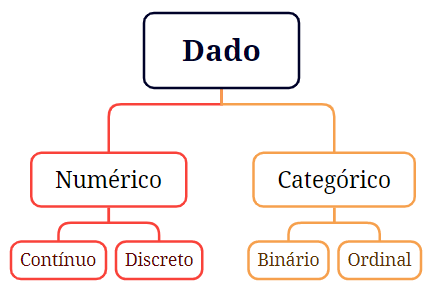
\includegraphics[width=2.64583in,height=\textheight]{figuras/tipo_dado.png}
\caption{Tipo do dado}
\end{figure}

Dado do tipo \textbf{numérico} é expresso geralmente expresso como um número inteiro ou real. Porém, existem casos em que números inteiros também expressam dados \textbf{categóricos}. Já o dado do tipo \textbf{categórico} está relacionado a um valor dentro de um lista (geralmente finita) de valores. A formação acadêmcia de uma determinada pessoa (Ensino Fundamental, Médio ou Superior), por exemplo, é um dado do tipo \textbf{categórico}. Já o salário, é um dado to tipo \textbf{númerico}.

\subsection{Numérico (ou quantitativo)}\label{numuxe9rico-ou-quantitativo}

O tipo do dado \textbf{numérico} ainda pode ser sub classificado como \textbf{numério} \textbf{contínuo} ou \textbf{númerico} \textbf{discreto}.

Um dado \textbf{numérico} \textbf{contínuo} é quando o dado pode ser qualquer número em um intervalo de números reais - lembrando que o conjunto de número reais engloba os números inteiros -. Geralmente é o resultado de uma medida, por exemplo, a altura dos estudantes é um dado do tipo \textbf{numérico} \textbf{contínuo}.

O dado \textbf{numérico discreto} geralmente é resultado de uma contagem - um número inteiro -, por exemplo, a idade é uma contagem de anos do estudante, é um dado \textbf{numérico discreto}.

Na nossa lista de idades, a idade é um dado do estudante do tipo \textbf{numérico discreto}.

\subsection{Categórico (ou qualitativo)}\label{categuxf3rico-ou-qualitativo}

Um dado é do tipo \textbf{categórico} representa um valor dentro de um conjunto ou de uma categoria.

O dado \textbf{categórico} pode ser \textbf{categótico binário} ou \textbf{categórito ordinal}, ou nenhuma das duas subcategorias, ou seja \textbf{categórico somente}.

Um exemplo de \textbf{dado categórico somente}, é uma lista com as cores preferidas dos estudantes (azul, verde, vermelho), ou o estado civil de uma pessoa (casado, solteiro).

O dado do tipo \textbf{categórico binário} é quando ele somente pode assumir dois valores no universo de valores possíveis. Por exemplo 0 ou 1, existente ou ausente, true ou false, sim e não.

O dado do tipo \textbf{categórico ordinal} é quando o valor é um elemento de um conjunto que pode ser ordenado, por exemplo, imagine a classificação de altura de estudantes onde somente os valores alto, médio e baixo são permitidos. Nesse exemplo, existe uma ordem, o aluno com altura classificado como baixo tem uma altura menor do que o aluno com altura média.

\begin{longtable}[]{@{}
  >{\raggedright\arraybackslash}p{(\columnwidth - 2\tabcolsep) * \real{0.4719}}
  >{\raggedright\arraybackslash}p{(\columnwidth - 2\tabcolsep) * \real{0.5281}}@{}}
\toprule\noalign{}
\begin{minipage}[b]{\linewidth}\raggedright
Variável
\end{minipage} & \begin{minipage}[b]{\linewidth}\raggedright
Tipo do dado
\end{minipage} \\
\midrule\noalign{}
\endhead
\bottomrule\noalign{}
\endlastfoot
Idade (Ex: 14, 17, 23) & numérico discreto \\
Doença (Ausente, Presente) & categório binário \\
Story Points (1, 3, 5, 7 \ldots{} ) & categorico ordinal \\
Ano (2021, 2022, \ldots) & numérico discreto \\
Altura (1,79 - 2,05 - \ldots) & numérico contínuo \\
Estado Civil (Casado, Solteiro) & categórico binário \\
Cores preferidas (Azul, verde, vermelho) & categórico somente (nem binário, nem ordinal) \\
\end{longtable}

Os dados geralmente são organizados em formato de tabelas. Onde as linhas representam as obseravações (ou instâncias) e as colunas representam as variáveis.

Vamos utilizar o exemplo de uma empresa que desenvolve software e registra os dados relacionados a seus projetos. Essa empresa mantem o registro de determinada funcionalidade e do tamanho dessa funcionalidade. Cada linha da tabela representa uma funcionalidade (chamada de User Story em projetos que utilizam SCRUM). Cada coluna representa uma informação dessa User Story. As informações que a empresa mantém registro são as variáveis, as colunas da tabela. Uma dessas variáveis é a descriçao, outra é uma estimativa que o desenvolvedor atribui do tamanho funional, chamado Story Point. Essas informações estão dispostas em um arquivo no formato CSV. O código abaixo, carrega esse arquivo e exibe parte de seu conteúdo. Iremos então classificar cada uma das colunas de acordo com o tipo do dado.

Código R

\begin{Shaded}
\begin{Highlighting}[]
\NormalTok{df }\OtherTok{\textless{}{-}} \FunctionTok{read\_csv}\NormalTok{(}\StringTok{\textquotesingle{}data/neodataset/7764.csv\textquotesingle{}}\NormalTok{)}
\end{Highlighting}
\end{Shaded}

\begin{verbatim}
## Rows: 355 Columns: 5
## -- Column specification --------------------------------------------------------
## Delimiter: ","
## chr  (2): title, description
## dbl  (2): issuekey, storypoints
## dttm (1): created
## 
## i Use `spec()` to retrieve the full column specification for this data.
## i Specify the column types or set `show_col_types = FALSE` to quiet this message.
\end{verbatim}

\begin{Shaded}
\begin{Highlighting}[]
\FunctionTok{head}\NormalTok{(df)}
\end{Highlighting}
\end{Shaded}

\begin{verbatim}
## # A tibble: 6 x 5
##   issuekey created             title                     description storypoints
##      <dbl> <dttm>              <chr>                     <chr>             <dbl>
## 1 29688087 2020-01-17 00:50:48 Update templates for web~ "Relates t~           1
## 2 29682716 2020-01-16 19:21:38 Make sure that we Captur~ "This was ~           1
## 3 29644971 2020-01-15 21:17:03 Propose new IA for Brand~ "## Goals\~           1
## 4 29494181 2020-01-10 19:20:50 Cache `node_modules` for~ "# UPDATE ~           1
## 5 29437529 2020-01-09 10:26:51 Disable all remaining un~ "Similar t~           1
## 6 29358963 2020-01-07 08:35:44 Disable unnecessary jobs~ "As discus~           1
\end{verbatim}

Código Python

\begin{Shaded}
\begin{Highlighting}[]
\ImportTok{import}\NormalTok{ pandas }\ImportTok{as}\NormalTok{ pd}
\CommentTok{\#pd.set\_option(\textquotesingle{}max\_columns\textquotesingle{}, None)}
\NormalTok{df }\OperatorTok{=}\NormalTok{ pd.read\_csv(}\StringTok{\textquotesingle{}data/neodataset/7764.csv\textquotesingle{}}\NormalTok{)}
\NormalTok{df.head()}
\end{Highlighting}
\end{Shaded}

\begin{verbatim}
##    issuekey  ... storypoints
## 0  29688087  ...           1
## 1  29682716  ...           1
## 2  29644971  ...           1
## 3  29494181  ...           1
## 4  29437529  ...           1
## 
## [5 rows x 5 columns]
\end{verbatim}

\begin{longtable}[]{@{}
  >{\raggedright\arraybackslash}p{(\columnwidth - 4\tabcolsep) * \real{0.1103}}
  >{\raggedright\arraybackslash}p{(\columnwidth - 4\tabcolsep) * \real{0.1379}}
  >{\raggedright\arraybackslash}p{(\columnwidth - 4\tabcolsep) * \real{0.7517}}@{}}
\toprule\noalign{}
\begin{minipage}[b]{\linewidth}\raggedright
Nome da Coluna
\end{minipage} & \begin{minipage}[b]{\linewidth}\raggedright
Tipo do dado
\end{minipage} & \begin{minipage}[b]{\linewidth}\raggedright
Observação
\end{minipage} \\
\midrule\noalign{}
\endhead
\bottomrule\noalign{}
\endlastfoot
Issuekey & categorico somente & Apesar de ser um número, não são realizadas operações no número, ele é um identificador único da User Story \\
stroypoints & numérico discreto & É um número geralmente de 1 á 100 \\
created & data & Data em que a User Story Foi criada \\
title & texto & Título da User Story \\
description & texto & Desrição da User Story \\
\end{longtable}

A tabela acima apresenta a caracterização dos dados do conjunto de dados neodataset (esse conjunto de dados pode ser baixado em \ldots). Nessa tabela foram tipificados os dados. É interessante apresentar essa tipificação em estudos cientificos e trabalhos de conclusão de curso, quando estamos lidando com conjuntos de dados. Cabe ressaltar que essa tipificação independe da linguagem. Internamente cada linguagem de programação tem seus tipos especificos e que podem ter pequenas diferenças entre as linguagens.

\section{Tipo do Atributo (Preditor, Alvo)}\label{tipo-do-atributo-preditor-alvo}

Nos modelos de aprendizagem de máquina (quando lidamos com algoritmos classificados como supervisionados) e de inferência estatistica o dado também pode ser classificado entre atributo preditor ou atributo alvo. Atributo preditor, são os atributos que serão utilizados para realizar a previsão, geralmente um ou mais atributos. Atributo alvo é o atributo que queremos `advinhar (ou dar o melhor chute técnico)' com os modelos preditivos. Atributo preditor muitas vezes é chamado de vairável independente, e atributo alvo de variável dependente.

\chapter{Análise exploratória dos dados}\label{anuxe1lise-exploratuxf3ria-dos-dados}

\section{Introdução}\label{introduuxe7uxe3o-1}

Um dos pioneiros na definição da área de análise exploratória de dados (em inglês Estatistical Data Analisys, ou EDA) foi Tukey (1997) \citep{tukey1977exploratory}. Tukey (1997) argumenta que seu foco, até aquele momento, estava em desenvolver novas técnicas para inferência. Porém, depois de reflexão, ele chega a conclusão de que o foco dele, e de outros estatísticos, seria melhor aplicado no desenvolvimento de técnicas para a etapa de preparação desses dados. Era nos procedimentos de estruturar os dados que estava o verdadeiro desafio. Problemas, tais como, lidar com dados faltantes ou \emph{outliers,} traziam impactos negativos na inferência e novas técnicas nessa etapa precisavam ser estudadas. Sua recomendação era uma mudança de paradigma e novos estudos, voltando mais para a preparação dos dados. Sua visão é de que isso iria trazer enorme avanços como um todo. O que de fato aconteceu.

Podemos considerar essa necessidade de estudos anterior ao processo de inferência analisando o exemplo criado por Ancobe.

R

\begin{Shaded}
\begin{Highlighting}[]
\NormalTok{x }\OtherTok{\textless{}{-}} \FunctionTok{c}\NormalTok{(}\DecValTok{10}\NormalTok{, }\DecValTok{8}\NormalTok{, }\DecValTok{13}\NormalTok{, }\DecValTok{9}\NormalTok{, }\DecValTok{11}\NormalTok{, }\DecValTok{14}\NormalTok{, }\DecValTok{6}\NormalTok{, }\DecValTok{4}\NormalTok{ , }\DecValTok{12}\NormalTok{, }\DecValTok{7}\NormalTok{, }\DecValTok{5}\NormalTok{)}
\NormalTok{y }\OtherTok{\textless{}{-}} \FunctionTok{c}\NormalTok{(}\FloatTok{8.04}\NormalTok{, }\FloatTok{6.95}\NormalTok{, }\FloatTok{7.58}\NormalTok{, }\FloatTok{8.81}\NormalTok{, }\FloatTok{8.33}\NormalTok{, }\FloatTok{9.96}\NormalTok{, }\FloatTok{7.24}\NormalTok{, }\FloatTok{4.26}\NormalTok{, }\FloatTok{10.84}\NormalTok{, }\FloatTok{4.82}\NormalTok{, }\FloatTok{5.68}\NormalTok{)}
\NormalTok{DT }\OtherTok{=} \FunctionTok{data.table}\NormalTok{(x, y)}
\FunctionTok{ggplot}\NormalTok{(DT, }\AttributeTok{mapping =} \FunctionTok{aes}\NormalTok{(}\AttributeTok{x =}\NormalTok{ x, }\AttributeTok{y =}\NormalTok{y)) }\SpecialCharTok{+}
  \FunctionTok{geom\_point}\NormalTok{() }\SpecialCharTok{+}
  \FunctionTok{labs}\NormalTok{(}\AttributeTok{title =} \StringTok{"Amostra 1"}\NormalTok{)}
\end{Highlighting}
\end{Shaded}

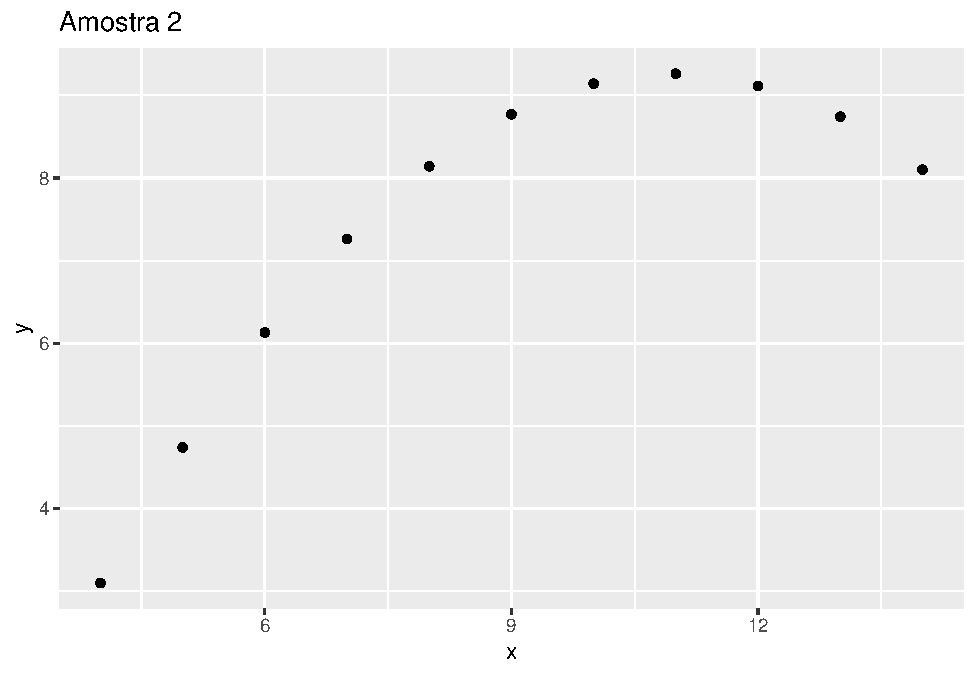
\includegraphics{_main_files/figure-latex/unnamed-chunk-11-1.pdf}

Python

\begin{Shaded}
\begin{Highlighting}[]
\ImportTok{import}\NormalTok{ matplotlib.pyplot }\ImportTok{as}\NormalTok{ plt}
\NormalTok{x }\OperatorTok{=}\NormalTok{ [}\DecValTok{10}\NormalTok{, }\DecValTok{8}\NormalTok{, }\DecValTok{13}\NormalTok{, }\DecValTok{9}\NormalTok{, }\DecValTok{11}\NormalTok{, }\DecValTok{14}\NormalTok{, }\DecValTok{6}\NormalTok{, }\DecValTok{4}\NormalTok{ , }\DecValTok{12}\NormalTok{, }\DecValTok{7}\NormalTok{, }\DecValTok{5}\NormalTok{]}
\NormalTok{y }\OperatorTok{=}\NormalTok{ [}\FloatTok{8.04}\NormalTok{, }\FloatTok{6.95}\NormalTok{, }\FloatTok{7.58}\NormalTok{, }\FloatTok{8.81}\NormalTok{, }\FloatTok{8.33}\NormalTok{, }\FloatTok{9.96}\NormalTok{, }\FloatTok{7.24}\NormalTok{, }\FloatTok{4.26}\NormalTok{, }\FloatTok{10.84}\NormalTok{, }\FloatTok{4.82}\NormalTok{, }\FloatTok{5.68}\NormalTok{]}
\NormalTok{plt.scatter(x, y)}
\NormalTok{plt.show()}
\end{Highlighting}
\end{Shaded}

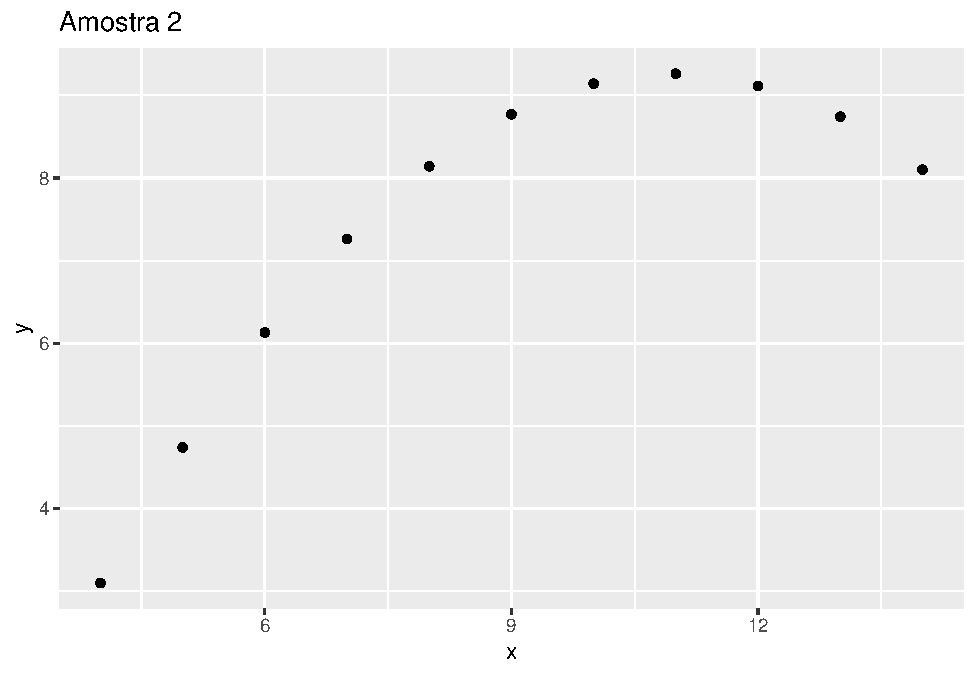
\includegraphics{_main_files/figure-latex/unnamed-chunk-12-1.pdf}

Veja a imagem ``Amostra 1'' acima. Nela visualmente percebemos uma relação linear direta entre as duas variáveis, podemos confirmar isso analisando o gráfico de pontos e o valor da correlação, abaixo.

R

\begin{Shaded}
\begin{Highlighting}[]
\FunctionTok{cor}\NormalTok{(x, y)  }
\end{Highlighting}
\end{Shaded}

\begin{verbatim}
## [1] 0.8164205
\end{verbatim}

Python

\begin{Shaded}
\begin{Highlighting}[]
\ImportTok{from}\NormalTok{ statistics }\ImportTok{import}\NormalTok{ correlation}
\BuiltInTok{print}\NormalTok{(correlation(x, y))}
\end{Highlighting}
\end{Shaded}

\begin{verbatim}
## 0.81642051634484
\end{verbatim}

Para os dados da Amostra 1, acima temos uma correlação de 0.81.

R

\begin{Shaded}
\begin{Highlighting}[]
\NormalTok{x }\OtherTok{\textless{}{-}} \FunctionTok{c}\NormalTok{(}\DecValTok{10}\NormalTok{, }\DecValTok{8}\NormalTok{, }\DecValTok{13}\NormalTok{, }\DecValTok{9}\NormalTok{, }\DecValTok{11}\NormalTok{, }\DecValTok{14}\NormalTok{, }\DecValTok{6}\NormalTok{, }\DecValTok{4}\NormalTok{ , }\DecValTok{12}\NormalTok{, }\DecValTok{7}\NormalTok{, }\DecValTok{5}\NormalTok{)}
\NormalTok{y }\OtherTok{\textless{}{-}} \FunctionTok{c}\NormalTok{(}\FloatTok{9.14}\NormalTok{, }\FloatTok{8.14}\NormalTok{, }\FloatTok{8.74}\NormalTok{,}\FloatTok{8.77}\NormalTok{,}\FloatTok{9.26}\NormalTok{,}\FloatTok{8.1}\NormalTok{,}\FloatTok{6.13}\NormalTok{,}\FloatTok{3.1}\NormalTok{,}\FloatTok{9.11}\NormalTok{,}\FloatTok{7.26}\NormalTok{,}\FloatTok{4.74}\NormalTok{)}
\NormalTok{DT }\OtherTok{=} \FunctionTok{data.table}\NormalTok{(x, y)}
\FunctionTok{ggplot}\NormalTok{(DT, }\AttributeTok{mapping =} \FunctionTok{aes}\NormalTok{(}\AttributeTok{x =}\NormalTok{ x, }\AttributeTok{y =}\NormalTok{y)) }\SpecialCharTok{+}
  \FunctionTok{geom\_point}\NormalTok{() }\SpecialCharTok{+}
  \FunctionTok{labs}\NormalTok{(}\AttributeTok{title =} \StringTok{"Amostra 2"}\NormalTok{)}
\end{Highlighting}
\end{Shaded}

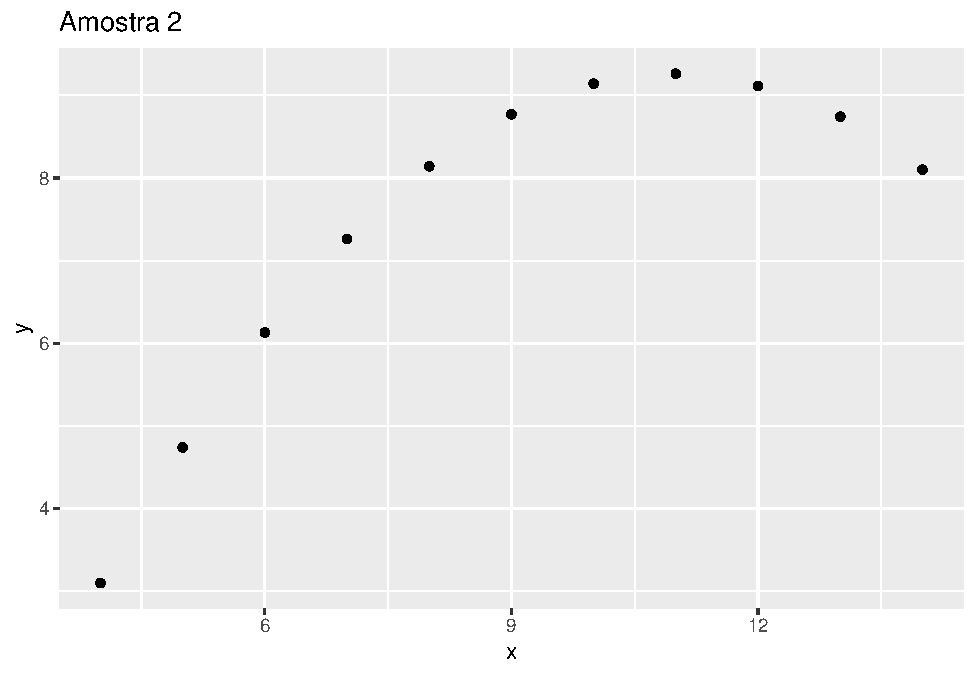
\includegraphics{_main_files/figure-latex/unnamed-chunk-15-1.pdf}

Python

\begin{Shaded}
\begin{Highlighting}[]
\ImportTok{import}\NormalTok{ matplotlib.pyplot }\ImportTok{as}\NormalTok{ plt}
\NormalTok{plt.plot([}\DecValTok{0}\NormalTok{, }\DecValTok{1}\NormalTok{, }\DecValTok{2}\NormalTok{, }\DecValTok{3}\NormalTok{])}
\NormalTok{plt.show()}
\end{Highlighting}
\end{Shaded}

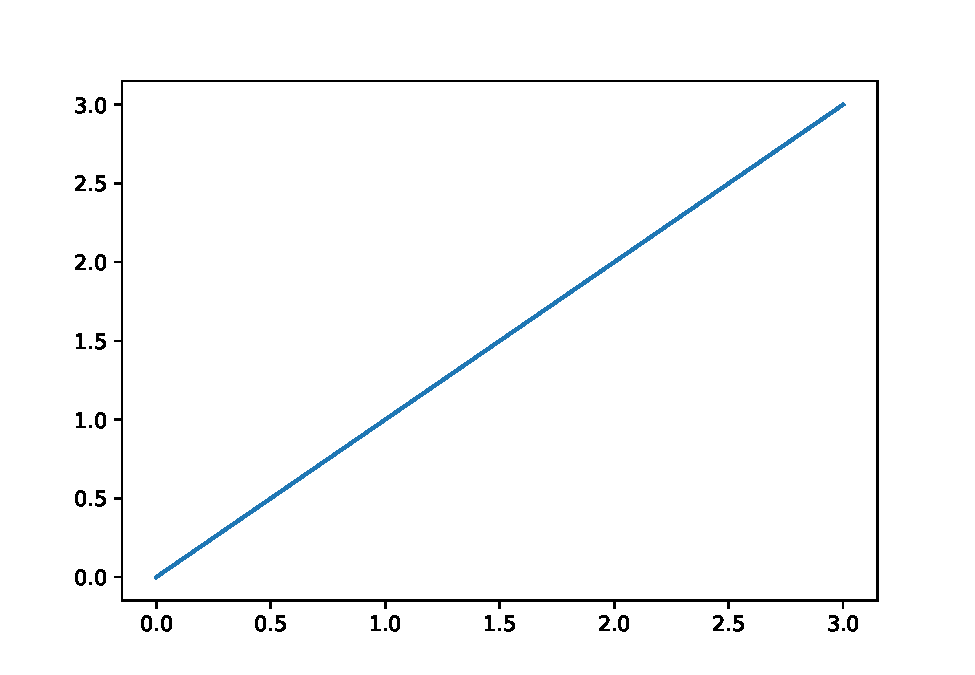
\includegraphics{_main_files/figure-latex/unnamed-chunk-16-1.pdf}

Na amostra 2 percebemos uma relação em forma de curva, quando verificamos a correlação verificamos o mesmo valor de 0.81 dos dados da amostra 1.

  \bibliography{book.bib,packages.bib}

\end{document}
